\documentclass[11pt]{article}
\usepackage[croatian]{babel}  % Croatian typographical rules and hyphenation patterns
\usepackage[utf8]{inputenc}  	% Encoding of Croatian characters
\usepackage[T1]{fontenc}
\usepackage{ae,aecompl}     	% Type 1 fonts, similar to Computer Modern

\usepackage{microtype}				% Improves spacing

\usepackage{booktabs}					% Nice looking tables
\usepackage{enumerate}				% Additional options for listing of items in enumerate environment
\usepackage{algorithm2e}			% Writing pseudo-code
\usepackage{todonotes}				% Adding todo items
\usepackage{dirtree}					% Simple display of directory tree
\usepackage{hyperref}
\usepackage{graphicx}
\usepackage{caption}
\graphicspath{ {./images/} }

\hypersetup{
    colorlinks=true,
    linkcolor=blue,
    filecolor=magenta,
    urlcolor=cyan,
}
\urlstyle{same}
\usepackage{graphics}
\title{
	\Large Sveučilište Josipa Jurja Strossmayera u Osijeku \\
	Fakultet elektrotehnike, računarstva i informacijskih tehnologija \\
	\vspace{4cm}
	\Large Kolegij: Linux u ugradbenim sustavima \\
	\vspace{4cm}
	\Large \textbf{Laboratorijska vježba 2: Upoznavanje s Raspberry Pi 3
	računalom. Izgradnja Linuxa za Raspberry Pi 3}
	}
\date{}
\begin{document}
\maketitle
\thispagestyle{empty}
\newpage

\section{Uvod}
Na tržištu se početkom 2012. godine pojavilo računalo Raspberry Pi i pokrenulo
 malu revoluciju u području obrazovanja i hobija vezanih za računalne znanosti.
 Ovo računalo je postalo izrazito popularno zbog svoje cijene (oko 35\$) i
 malih dimenzija (8,6cm x 5,4cm x 1,7cm). Iako je Raspberry Pi računalo opće
 namjene, ima mogućnost priključivanja različite opreme (npr. različiti senzori
 i aktuatori) pa se koristi u mnogim hobi projektima u području ugradbenih
 računalnih sustava i interneta objekata, a sve češće i u različitim
 komercijalnim projektima. Glavni dio ovog računala predstavlja SoC (engl.
 \textit{System On a Chip}) uz koji se nalazi različita periferija poput RAM
 memorije, HDMI izlaza, Ethernet priključka i sl. Također, na pločici se
 nalaze i pinovi koji predstavljaju ulazno izlazne pinove opće namjene (engl.
 \textit{General Purpose Input Output - GPIO}) koji omogućuje spajanje, u
 svijetu PC-a, nestandardne opreme.

\section{Modeli Raspberry Pi računala}
Do danas je na tržište izašlo nekoliko generacija Raspberry Pi računala.
Svima je zajednički Broadcom SoC s integriranim ARM procesorom (CPU) i
 ugrađenim grafičkim procesorom (GPU).
Brzina takta procesora se kreće od 700 MHz do 1.4 GHz kod modela Pi 3B+ ili
 1.5 GHz kod modela Pi 4. Količina memorije (RAM) se kreće od 256 MB do 1 GB
 ili čak 4 GB kod najjačeg modela najnovijeg Pi 4. \textit{Secure Digital} (SD)
 kartice se koriste za pohranu operativnog sustava i programa. Na pločama se
 nalaze do četiri USB priključka. Za video izlaz koristi se HDMI.
 Pomoću GPIO pinova podržani su standardni protokoli kao što je
 I\textsuperscript{2}C.
Svi B modeli imaju \textit{Ethernet} priključak, dok modeli Pi 3 i Pi Zero W
imaju \textit{Wi-Fi 802.11n} te \textit{Bluetooth}.
\newline
\newline
\textbf{Raspberry Pi Zero} manjih dimenzija i s reduciranim brojem
 ulazno-izlaznih jedinica te ulazno-izlaznih jedinica opće namjene (GPIO) je
 izašao na tržište 2015. godine s cijenom od 5\$. 2017. godine izlazi
 \textbf{Raspberry Pi Zero W} s dodanim \textit{Wi-Fi} i \textit{Bluetooth}
 mogućnostima.
\begin{figure}[h!]
\centering
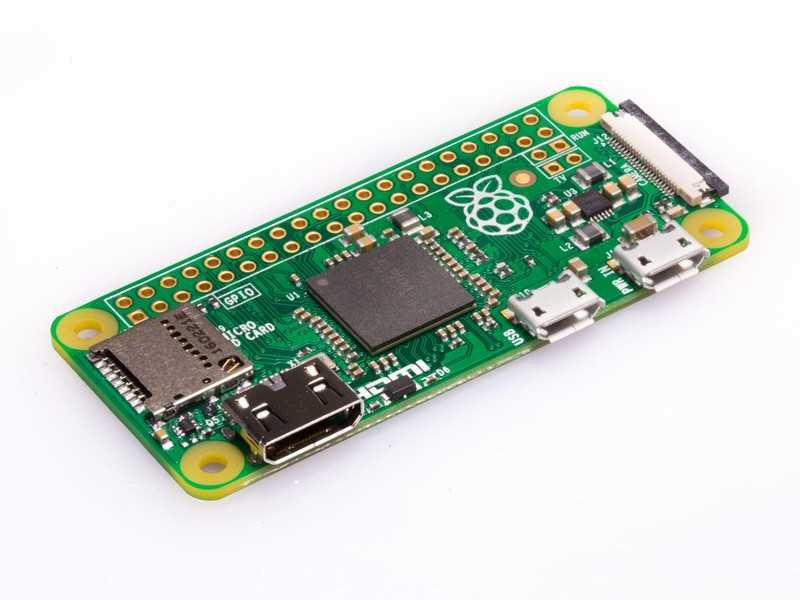
\includegraphics[width=0.8\textwidth]{rpi-zero.jpg}
\captionsetup{justification=centering}
\caption{Raspberry Pi Zero}
\end{figure}
\newline
\textbf{Raspberry Pi 3 Model B} je izašao 2016. godine s 1.2 GHz 64-bitnim
 četverojezgrenim procesorom te ugrađenim 802.11n Wi-Fi i Bluetooth mrežnim
 mogućnostima. 2018. godine izlazi \textbf{Raspberry Pi 3 Model B+} s 1.4 GHz
 procesorom te gigabitnom \textit{Ethernet} mrežom ne punih mogućnosti (u
 stvarnim testovima dostiže brzinu 300 Mbit/s, jer dijeli USB 2.0 sabirnicu).
 Posjeduje \textit{dual-band 802.11ac 2.4/5 Ghz Wi-Fi} bežični mrežni standard.
\newline
\newline
 Najnoviji model izlazi 2019. godine. Radi se o modelu \textit{Raspberry Pi
 4 Model B}. Hardverski definitivno najjači model Raspberry Pi računala s
 1.5 GHz četverojezgrenim \textbf{ARM Cortex-A72} procesorom, podrškom za
 802.11ac Wi-Fi bežičnom mrežom, \textbf{Bluetooth 5} podrškom,
 podrškom za gigabitnom Ethernet mrežom punih mogućnosti, dva \textbf{USB 2.0}
 porta, dva \textbf{USB 3.0} porta te podrškom za \textbf{4K} video rezolucijom.
\begin{figure}[h!]
\centering
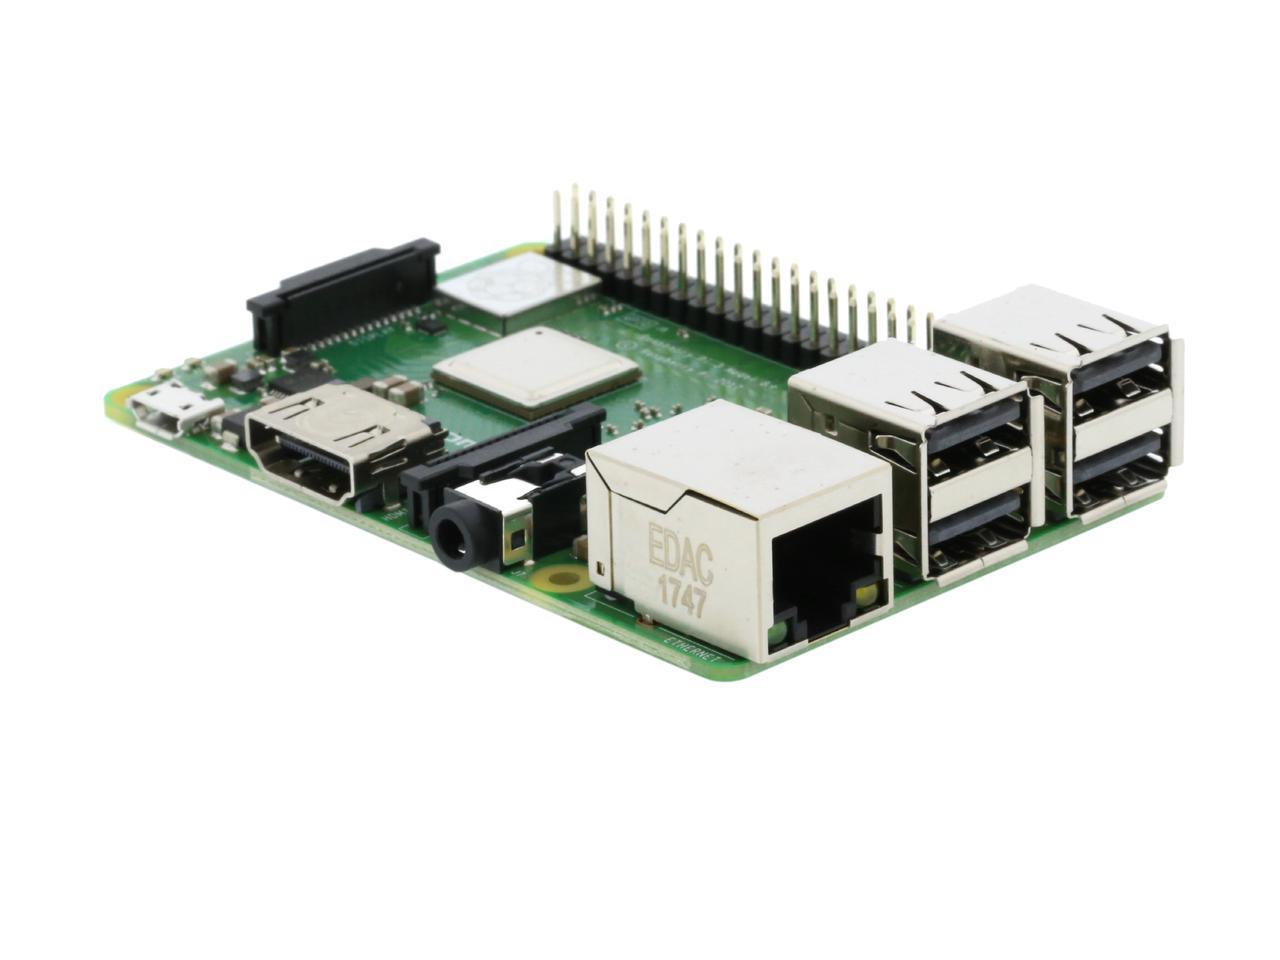
\includegraphics[width=0.8\textwidth]{rpi-3-b-plus.jpg}
\captionsetup{justification=centering}
\caption{Raspberry Pi 3 B+}
\end{figure}
\begin{figure}[h!]
\centering
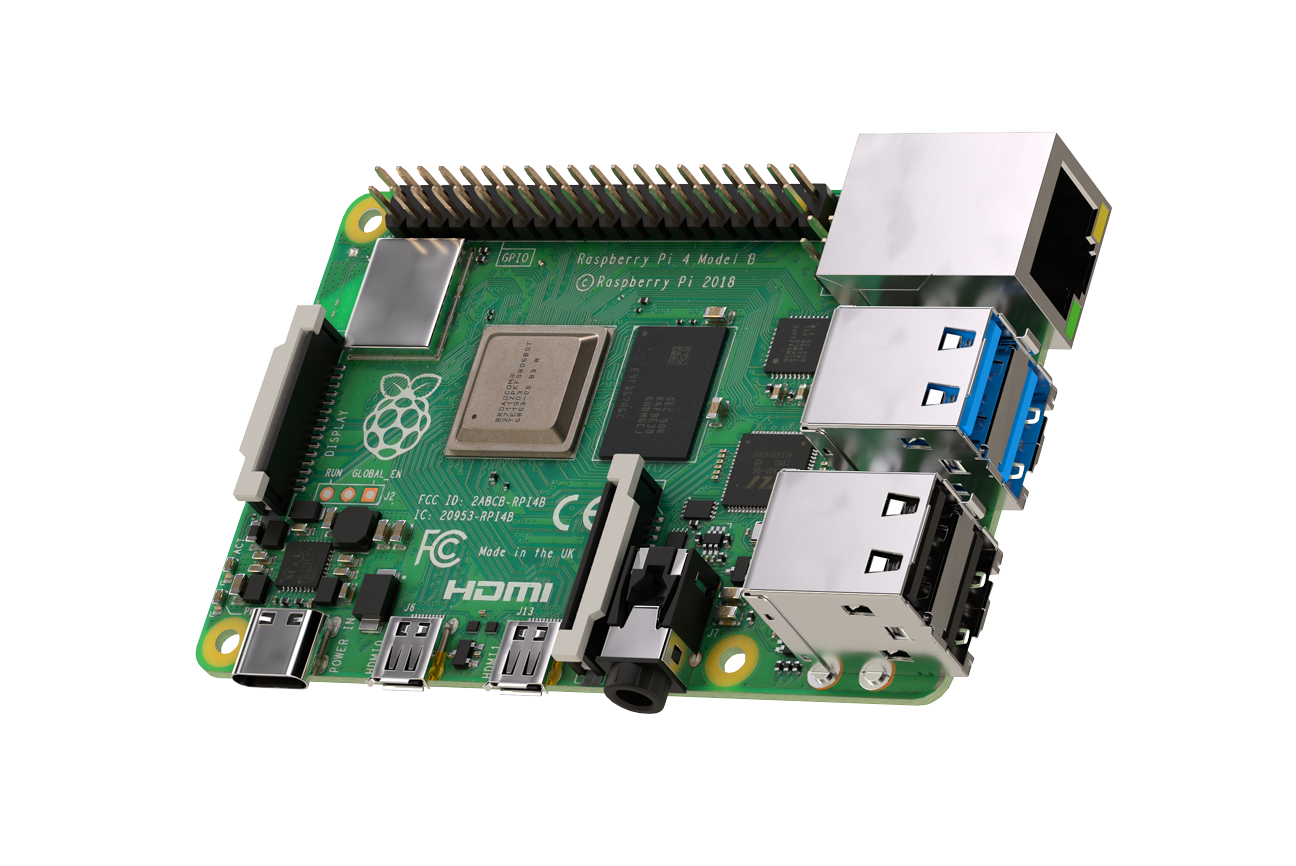
\includegraphics[width=0.8\textwidth]{rpi-4.png}
\captionsetup{justification=centering}
\caption{Raspberry Pi 4 B}
\end{figure}
\newline
\newline
Na laboratorijskim vježbama će se koristiti \textbf{Raspberry Bi 3 B}.
\newline
\newline
Tehničke karakteristike Raspberry Pi 3 B: \\
\textbf{SoC}: Broadcom BCM2837 \\
\textbf{CPU}: četverojezgreni ARM Cortex-A53, 1.2GHz \\
\textbf{GPU}: Broadcom VideoCore IV \\
\textbf{RAM}: 1GB LPDDR2 (900 MHz) \\
\textbf{Mreža}: 10/100 Ethernet, 2.4GHz 802.11n wireless \\
\textbf{Bluetooth}: Bluetooth 4.1 Classic, Bluetooth Low Energy \\
\textbf{Pohrana}: microSD \\
\textbf{GPIO}: 40-pin header, populated \\
\textbf{Priključci}: $4\times USB 2.0$, HDMI, 3.5mm analogni priključak,
 Ethernet, \textit{Camera Serial Interface} (CSI), \textit{Display Serial
 Interface} (DSI)
\begin{figure}[h!]
\centering
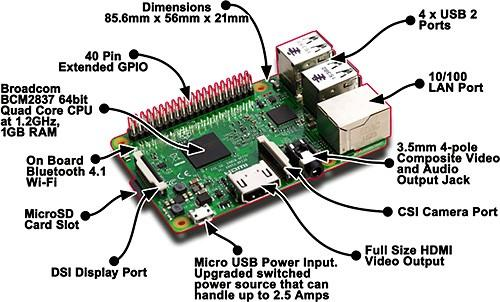
\includegraphics[width=0.8\textwidth]{rpi-3-details.jpg}
\captionsetup{justification=centering}
\caption{Raspberry Pi 3 detalji}
\end{figure}
\begin{figure}[h!]
\centering
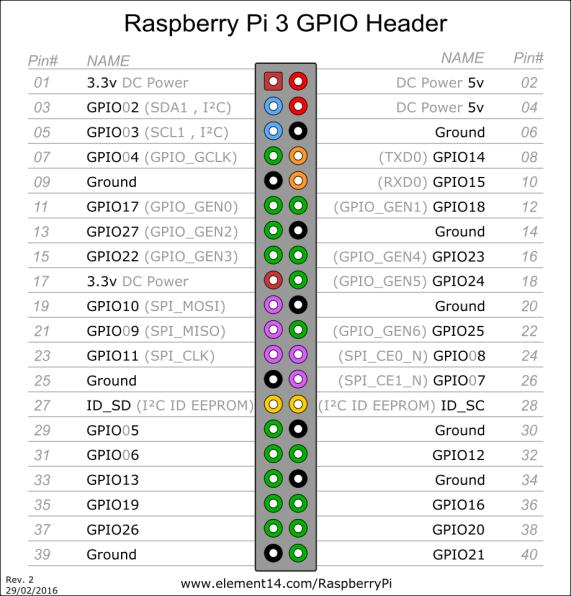
\includegraphics[width=0.8\textwidth]{rpi-3-pins.jpg}
\captionsetup{justification=centering}
\caption{Raspberry Pi 3 GPIO raspored}
\end{figure}
\end{document}
